\documentclass[answers]{exam}
%\documentclass{exam}

\usepackage{xeCJK}
\usepackage{zhnumber}
\usepackage{graphicx}
\usepackage{hyperref}
\usepackage{amsmath}
\usepackage{booktabs}
\usepackage{enumerate}

\pagestyle{headandfoot}
\firstpageheadrule
\firstpageheader{南京大学}{数字信号处理}{习题集三}
\runningheader{南京大学}
{数字信号处理}
{习题集三}
\runningheadrule
\firstpagefooter{}{第\thepage\ 页(共\numpages 页)}{}
\runningfooter{}{第\thepage\ 页(共\numpages 页)}{}

% no box for solutions
% \unframedsolutions

\setlength\linefillheight{.5in}

% \renewcommand{\solutiontitle}{\noindent\textbf{答:}}
\renewcommand{\solutiontitle}{\noindent\textbf{解:}\par\noindent}

\renewcommand{\thequestion}{\zhnum{question}}
\renewcommand{\questionlabel}{\thequestion .}
\renewcommand{\thepartno}{\arabic{partno}}
\renewcommand{\partlabel}{\thepartno .}


\begin{document}
\Large

\begin{questions}



\question 如图~\label{fig:q1-1}所示的系统,带通滤波器的频率响应如图~\label{fig:q1-2}所示,其相频特性$\phi(\omega)=0$,若输入$f(t)=\frac{\sin 2t}{2\pi t}$,$s(t)=\cos 1000t$,求输出信号$y(t)$。
\begin{figure}
	\centering
	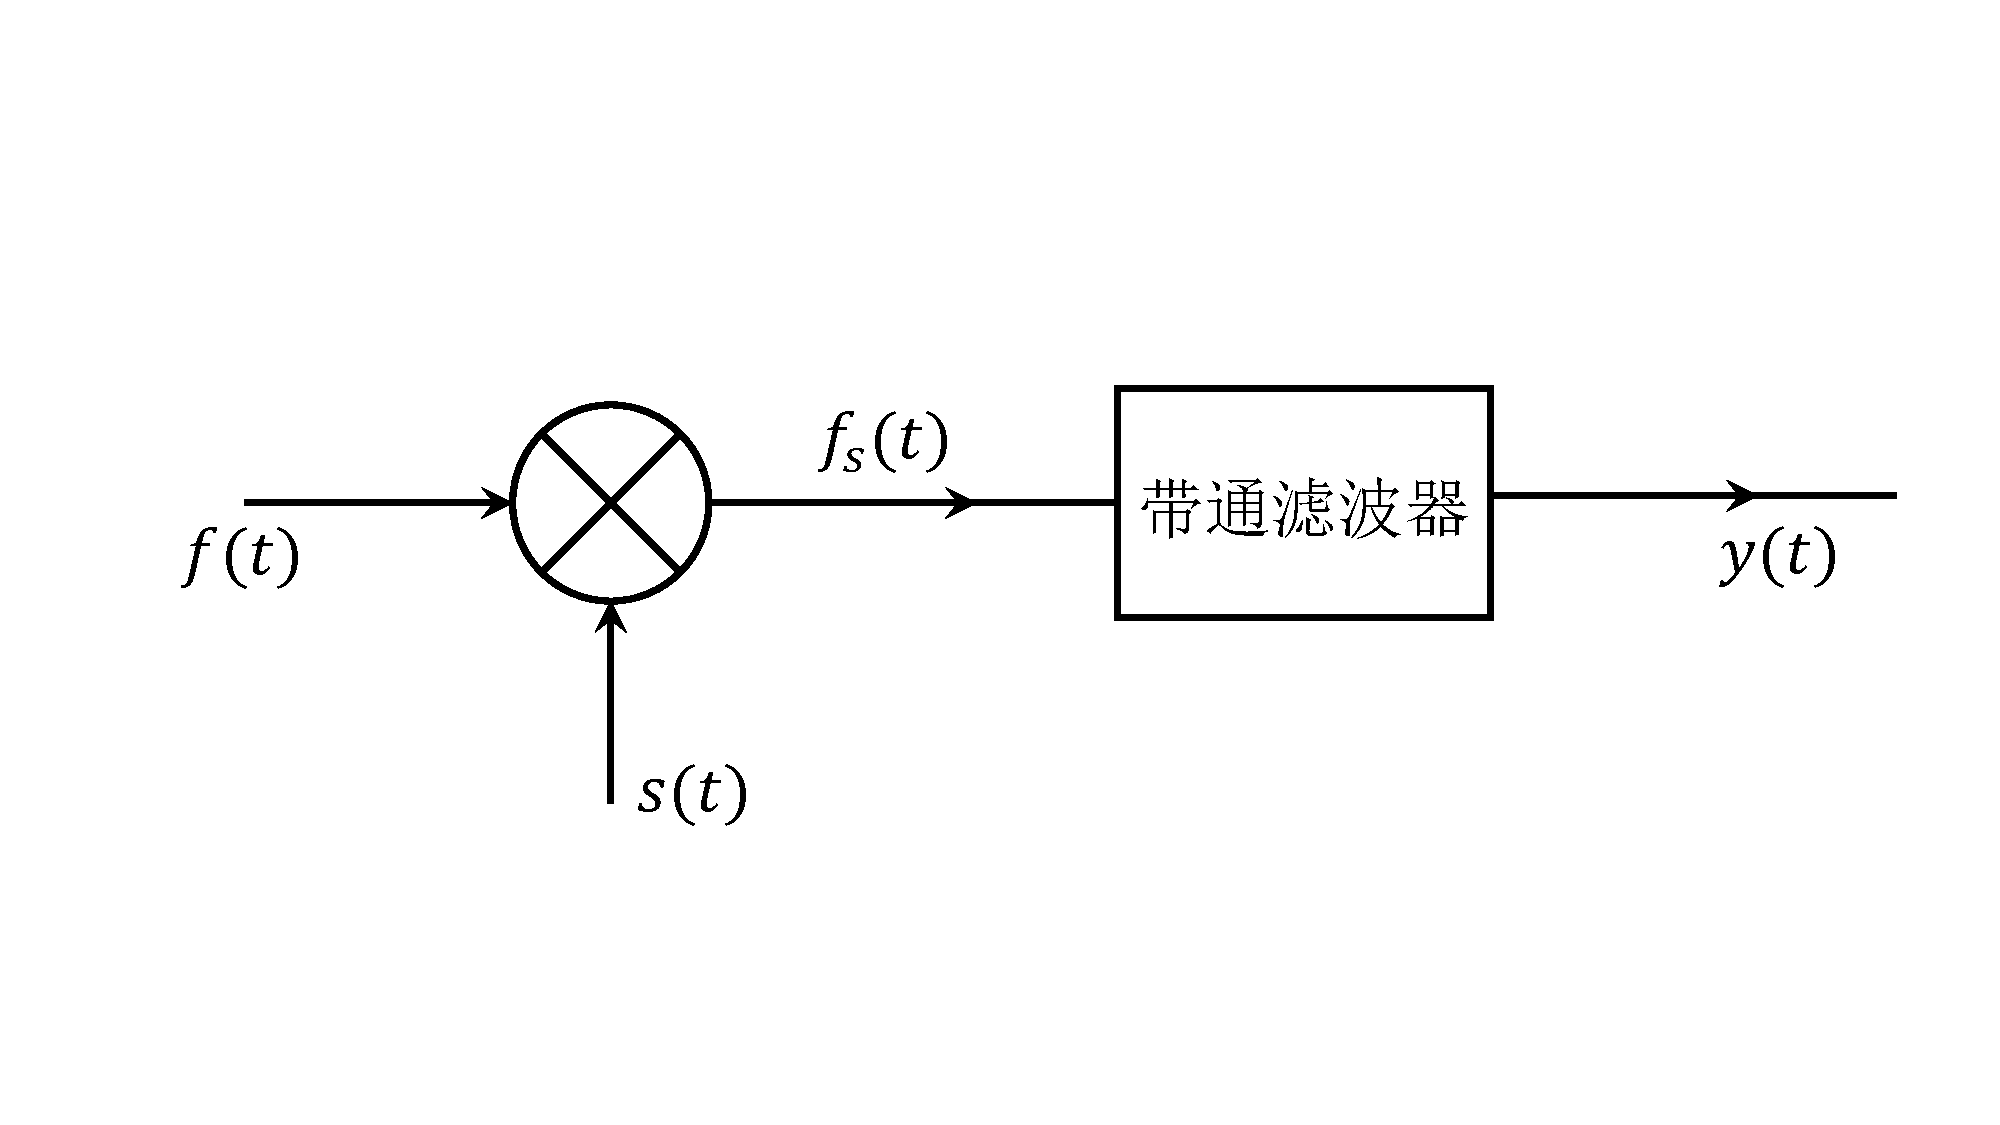
\includegraphics[width=0.8\textwidth]{pics/q1-1.pdf}
	\caption{第一题图(a)}
	\label{fig:q1-1}
\end{figure}
\begin{figure}
	\centering
	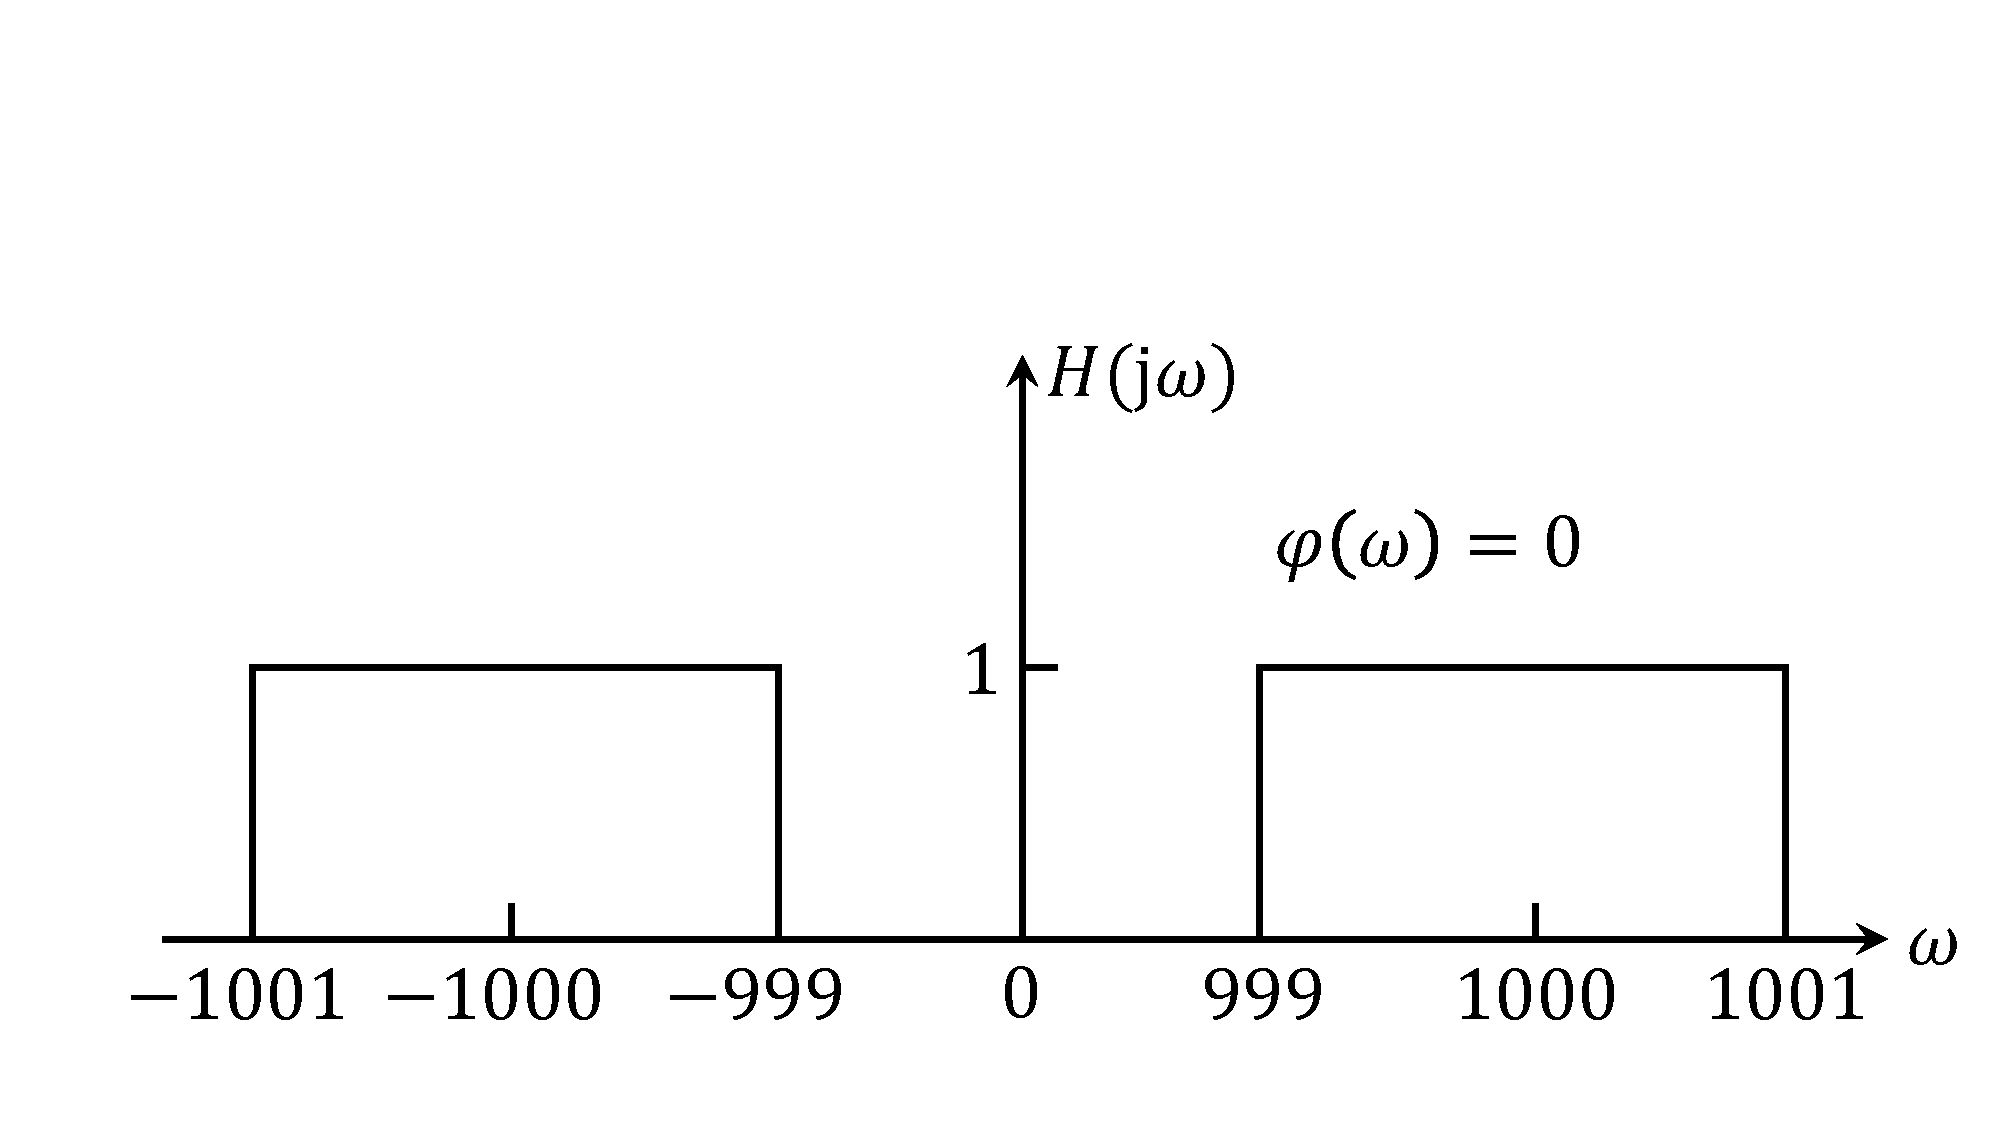
\includegraphics[width=0.8\textwidth]{pics/q1-2.pdf}
	\caption{第一题图(b)}
	\label{fig:11-2}
\end{figure}

\begin{solution}
	记$\mathcal{F}[f(t)]=X(jw)$,$\mathcal{F}[\frac{sint}{t}]=X_1(jw)$
\begin{align*}
	X(jw)=&F[\frac{sin2t}{2\pi t}]\\
	&=\frac{1}{\pi}\mathcal{F}[\frac{sin2t}{2t}]\\
	&=\frac{1}{\pi}\cdot\frac{1}{2}X_1(\frac{jw}{2})\\
	&=\frac{1}{2}[u(1-0.5w)-u(-1-0.5w)]
\end{align*}
故
\begin{align*}
	\mathcal{F}[f_s(t)]&=\frac{1}{2\pi}[\mathcal{F}[f(t)]*\mathcal{F}[s(t)]]\\
	&=\frac{1}{2}[X(j(w+1000))+X(j(w-1000))]
\end{align*}
我们可以绘制出$\mathcal{F}[f_s(t)]$的图像,经过带通滤波器后,两边都只保留中间的一半,即
$$Y(jw)=\frac{1}{4}\{[u(-999-w)-u(-1001-w)]+[u(1001-w)-u(999-w)]\}$$
对$Y(jw)$作傅里叶反变换\\
\begin{align*}
	y(t)&=\frac{1}{2\pi}\int_{-\infty}^{\infty}Y(jw)e^{jwt}dw\\
	&=\frac{1}{8\pi}[\int_{-1001}^{-999}e^{jwt}dw+\int_{999}^{1001}e^{jwt}dw]\\
	&=\frac{1}{4\pi}\frac{sin(1001t)-sin(999t)}{t}
\end{align*}
\end{solution}
\begin{figure}[h]
	\centering
	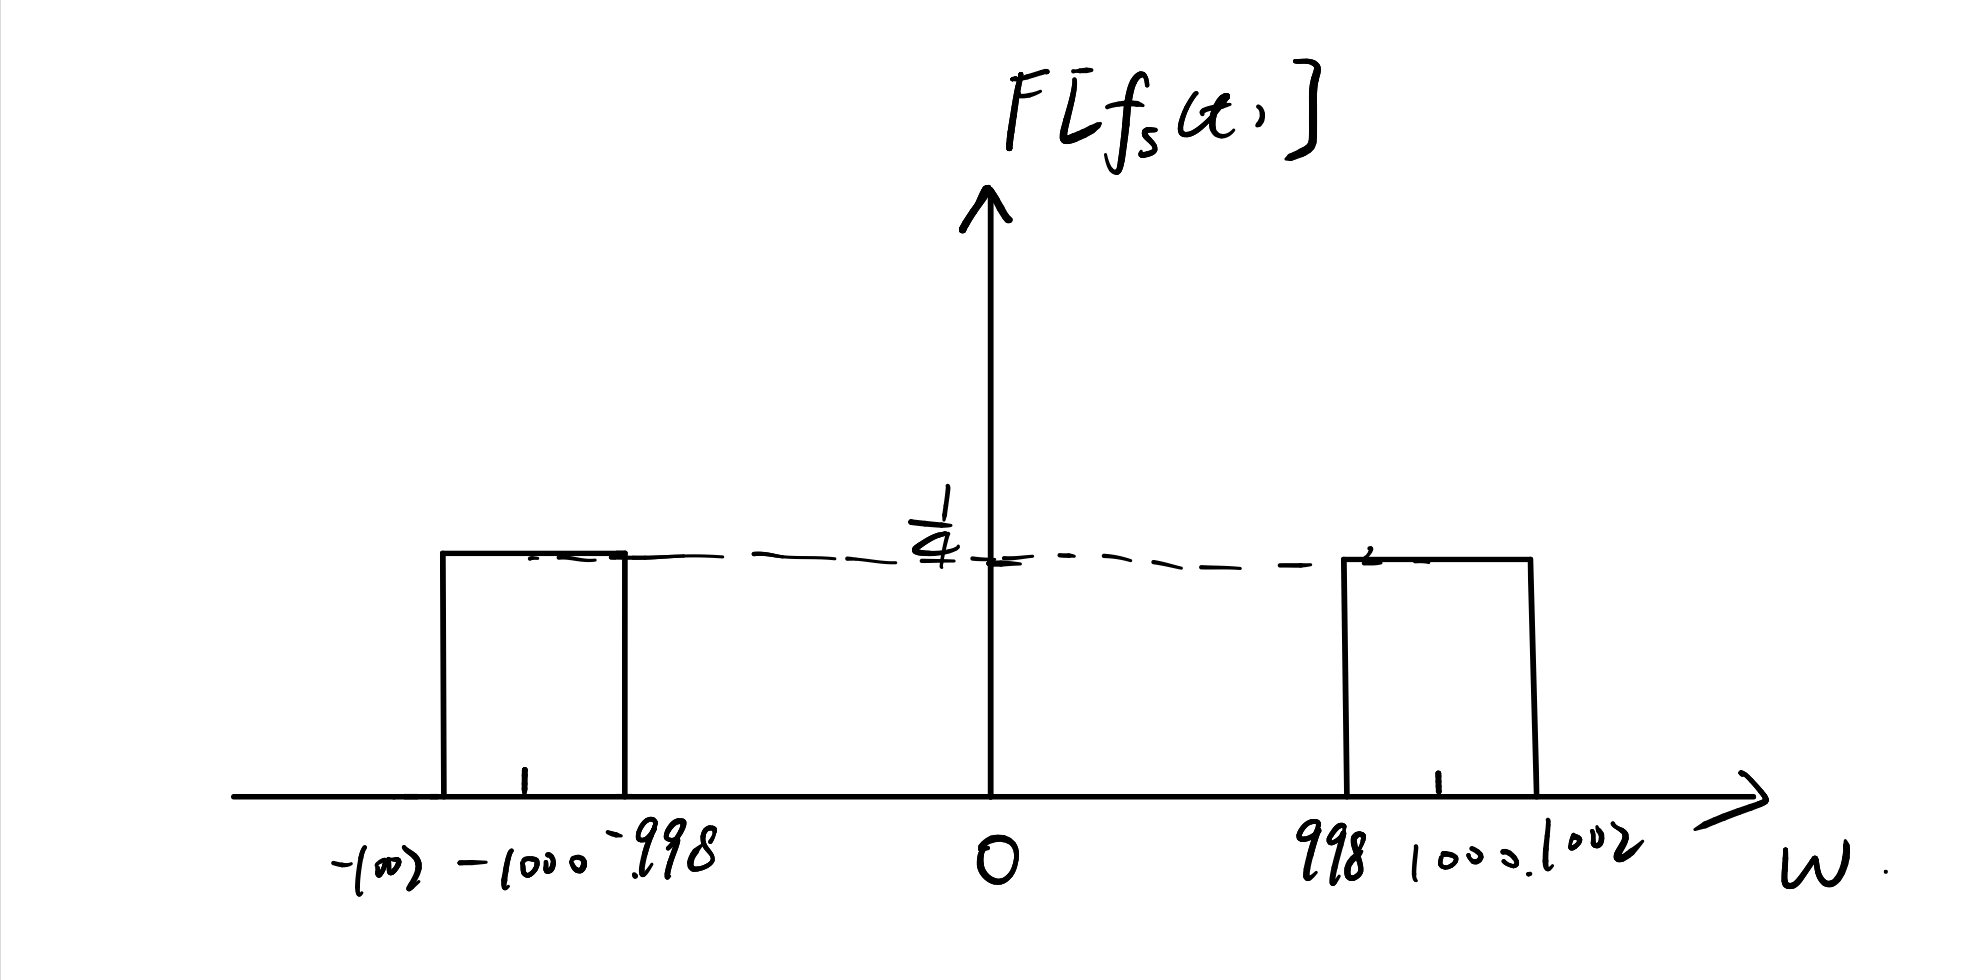
\includegraphics[width=0.8\textwidth]{pics/p1.png}
	\caption{$\mathcal{F}[f_s(t)]$}
\end{figure}

\newpage
\question 若$x(t)=\cos(\omega_{m}t)$,$\delta_{T}(t)=\sum_{n=-\infty}^{\infty}\delta(t-nT)$,$T=\frac{2\pi}{\omega_{s}}$,分别画出以下情况$x(t)\cdot\delta_{T}(t)$波形及其频谱$\mathcal{F}[x(t)\delta_{T}(t)]$图形。讨论从$x(t)\delta_{T}(t)$能否恢复$x(t)$。注意比较(1)和(4)的结果。(建议画波形时保持$T$不变)。
\begin{enumerate}[(1)]
\item $\omega_{m}=\frac{\omega_{s}}{8}=\frac{\pi}{4T}$
\item $\omega_{m}=\frac{\omega_{s}}{4}=\frac{\pi}{2T}$
\item $\omega_{m}=\frac{\omega_{s}}{2}=\frac{\pi}{T}$
\item $\omega_{m}=\frac{9\omega_{s}}{8}=\frac{9\pi}{4T}$
\end{enumerate}
~\\
解:为排版方便,在此页后四页放置各小问图片\\
本页讨论能否恢复,并给出$\mathcal{F}[x(t)]=\pi[\delta(w+w_m)+\delta(w-w_m)]$的图像\\
~\\
(1)能,由采样定理$w_s>2w_m$\\
~\\
(2)能,因为$w_s>2w_m$\\
~\\
(3)不能,$w_s=2w_m$,导致发生混叠\\
~\\
(4)不能,$w_s<2w_m$\\
\begin{figure}[h]
	\centering
	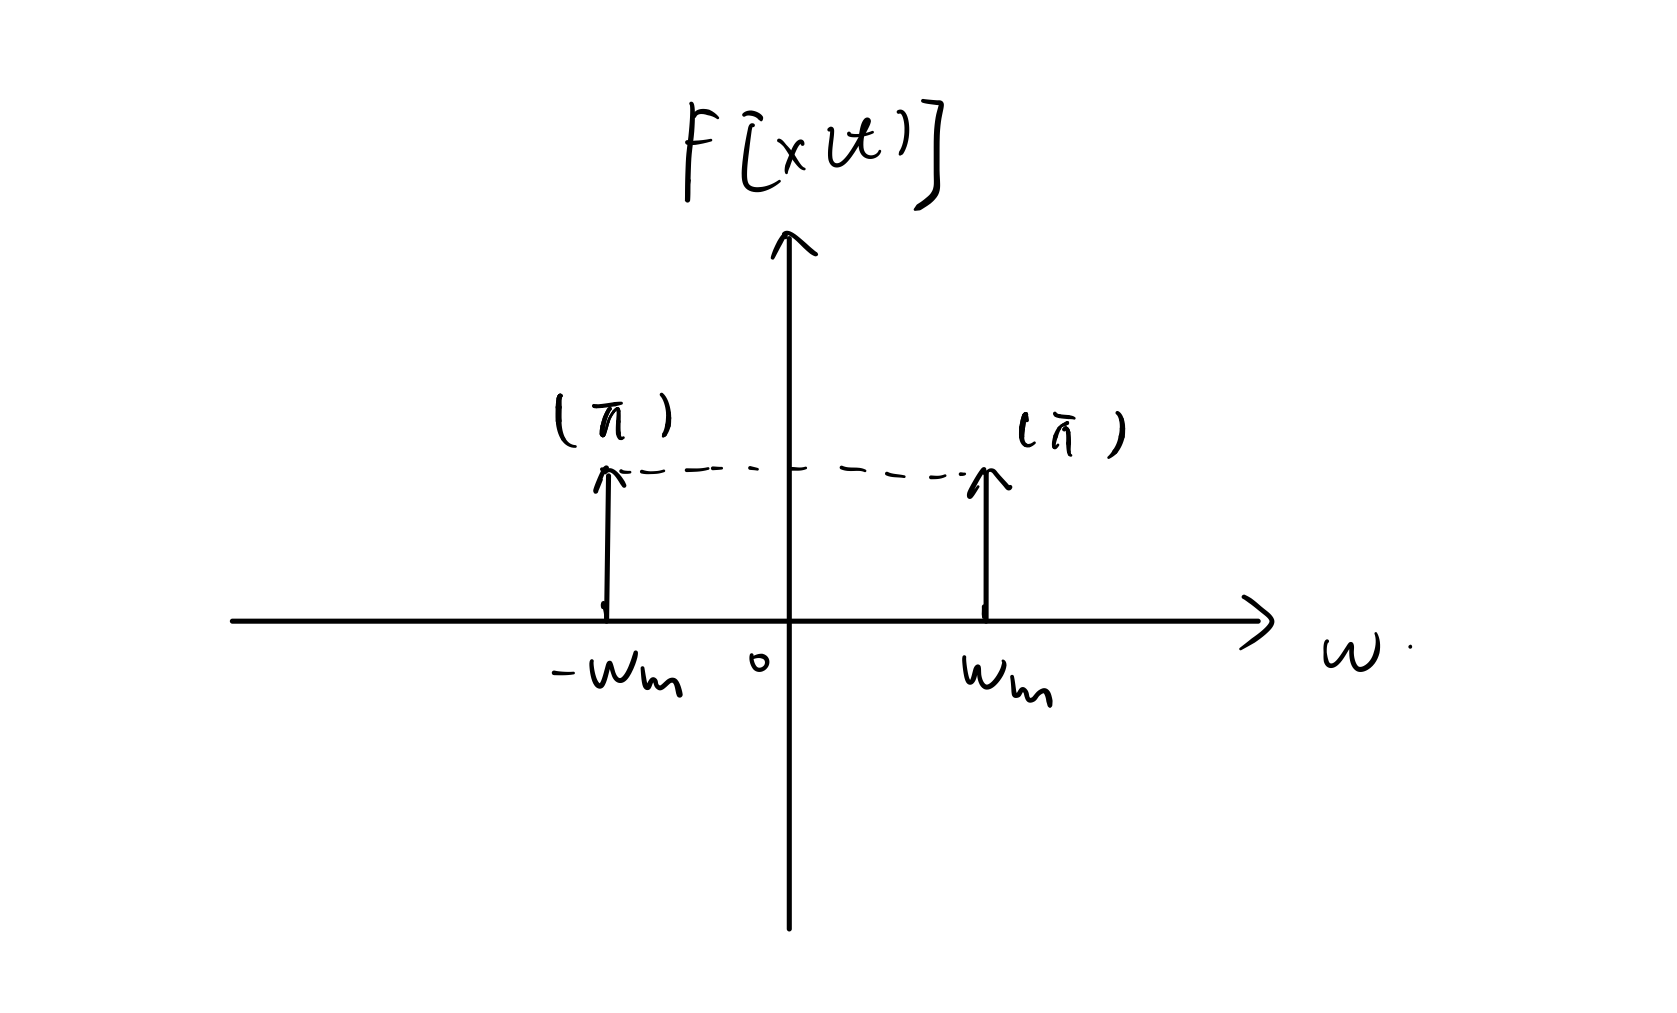
\includegraphics[width=0.8\textwidth]{pics/p2-0.PNG}
	\caption{$\mathcal{F}[x(t)]$}
\end{figure}
\newpage
(1)、$x(t)$周期$T_0=\frac{2\pi}{w_m}=8T$,图片如下:\\
\begin{figure}[h]
	\centering
	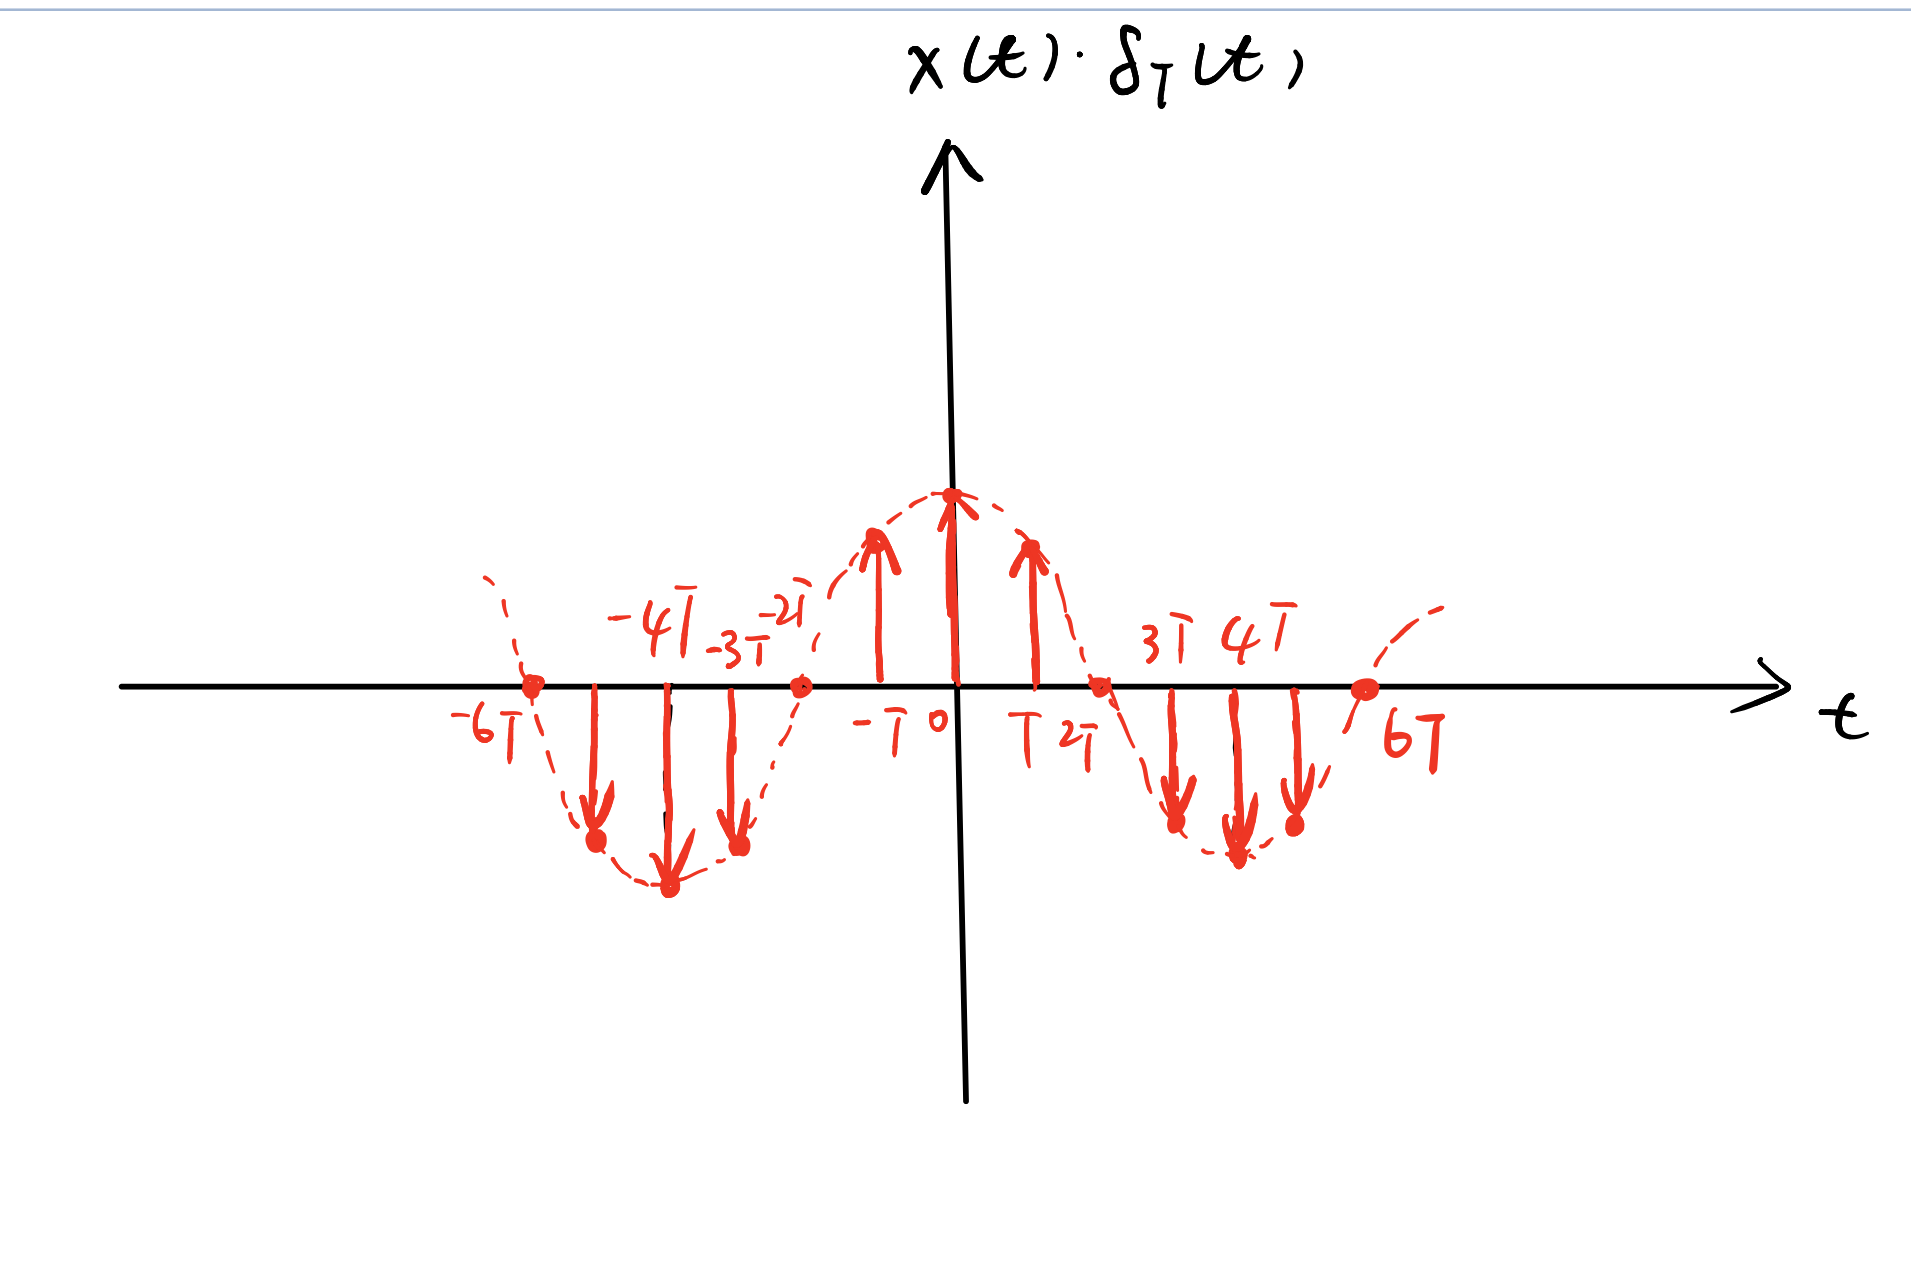
\includegraphics[width=0.8\textwidth,height=7.5cm]{pics/p2-1-1.PNG}
	\caption{(1)$x(t)\cdot\delta_T(t)$}
\end{figure}
\begin{figure}[h]
	\centering
	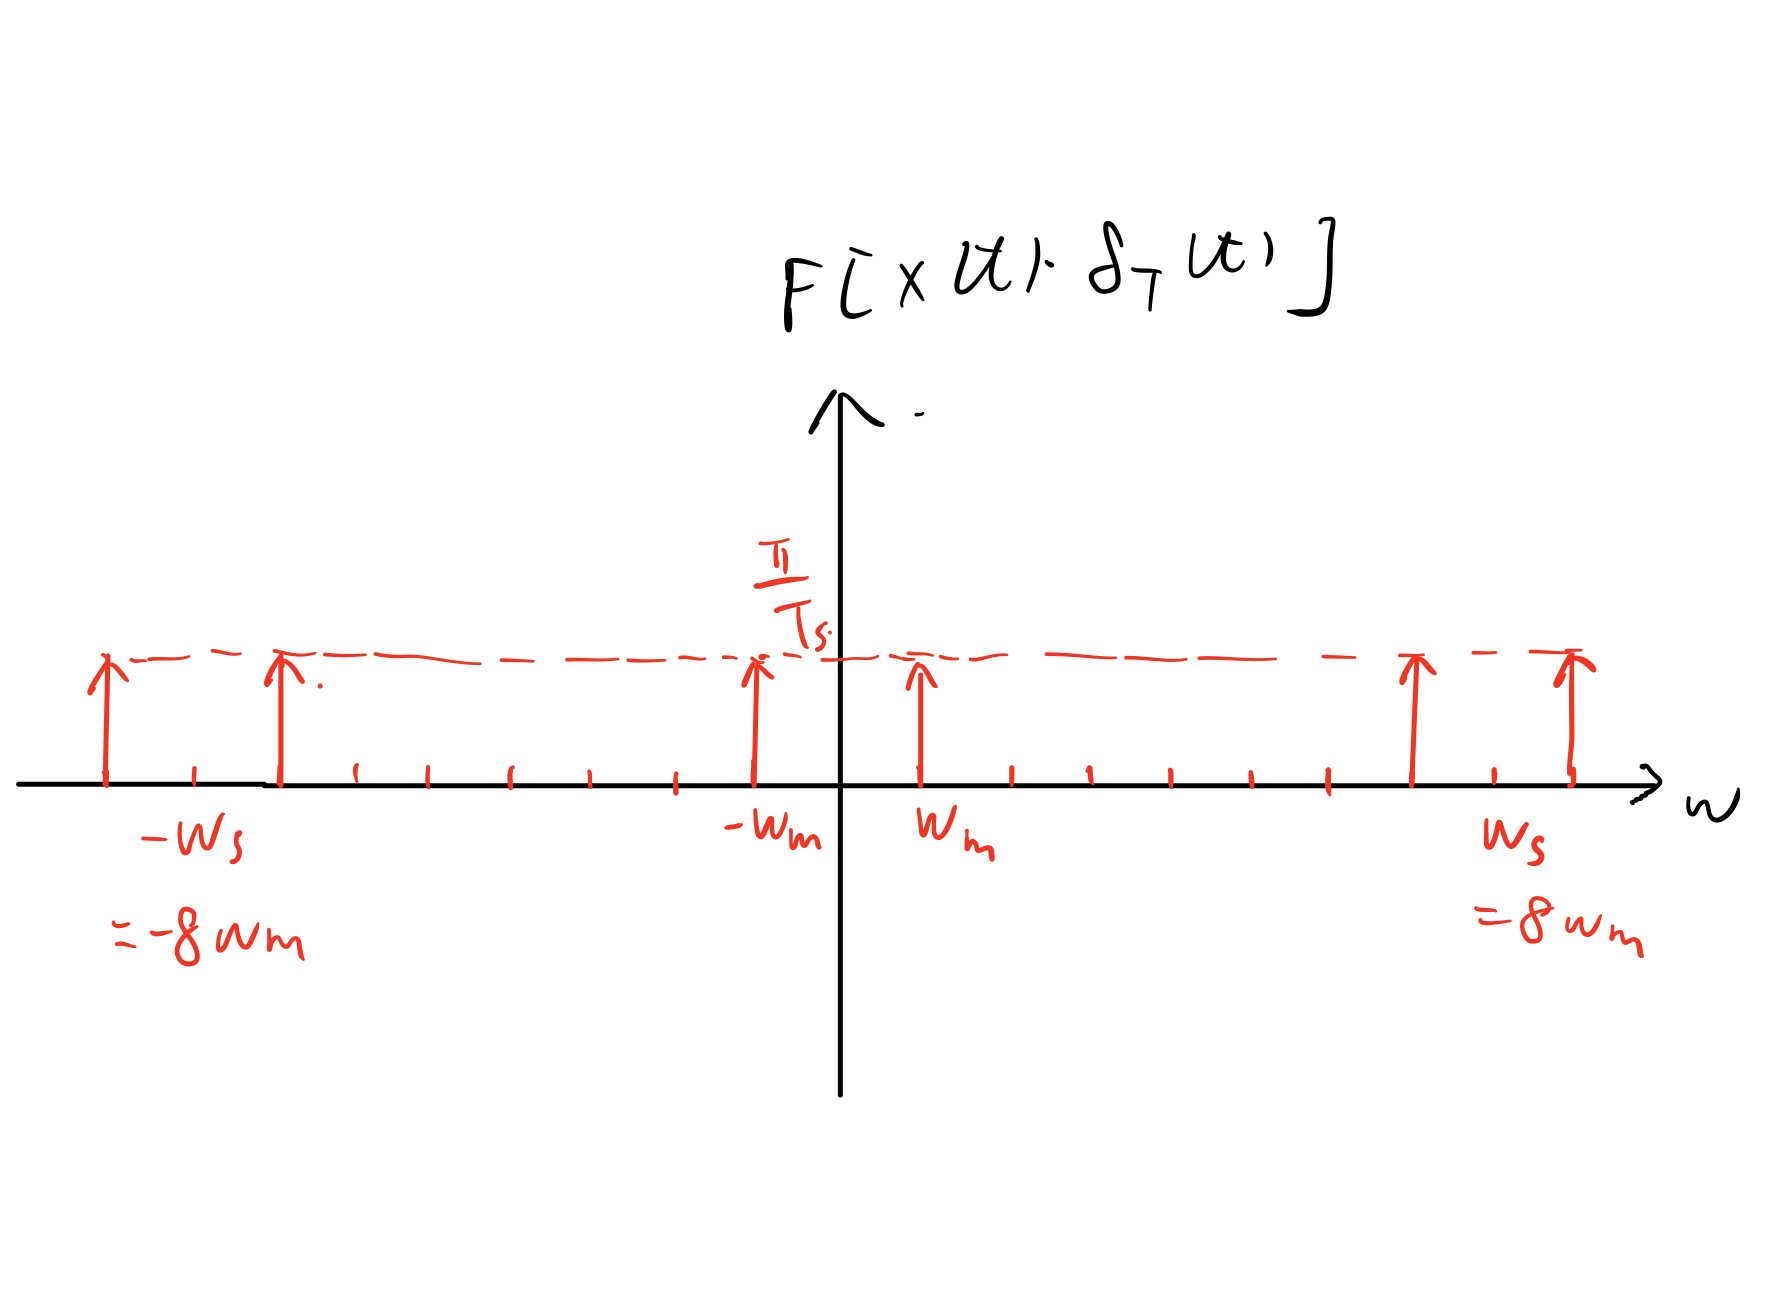
\includegraphics[width=0.8\textwidth,height=7cm]{pics/p2-1-2.PNG}
	\caption{(1)$\mathcal{F}[x(t)\delta_T(t)]$}
\end{figure}


\newpage
(2)、$x(t)$周期$T_0=\frac{2\pi}{w_m}=4T$,图片如下:\\
\begin{figure}[h]
	\centering
	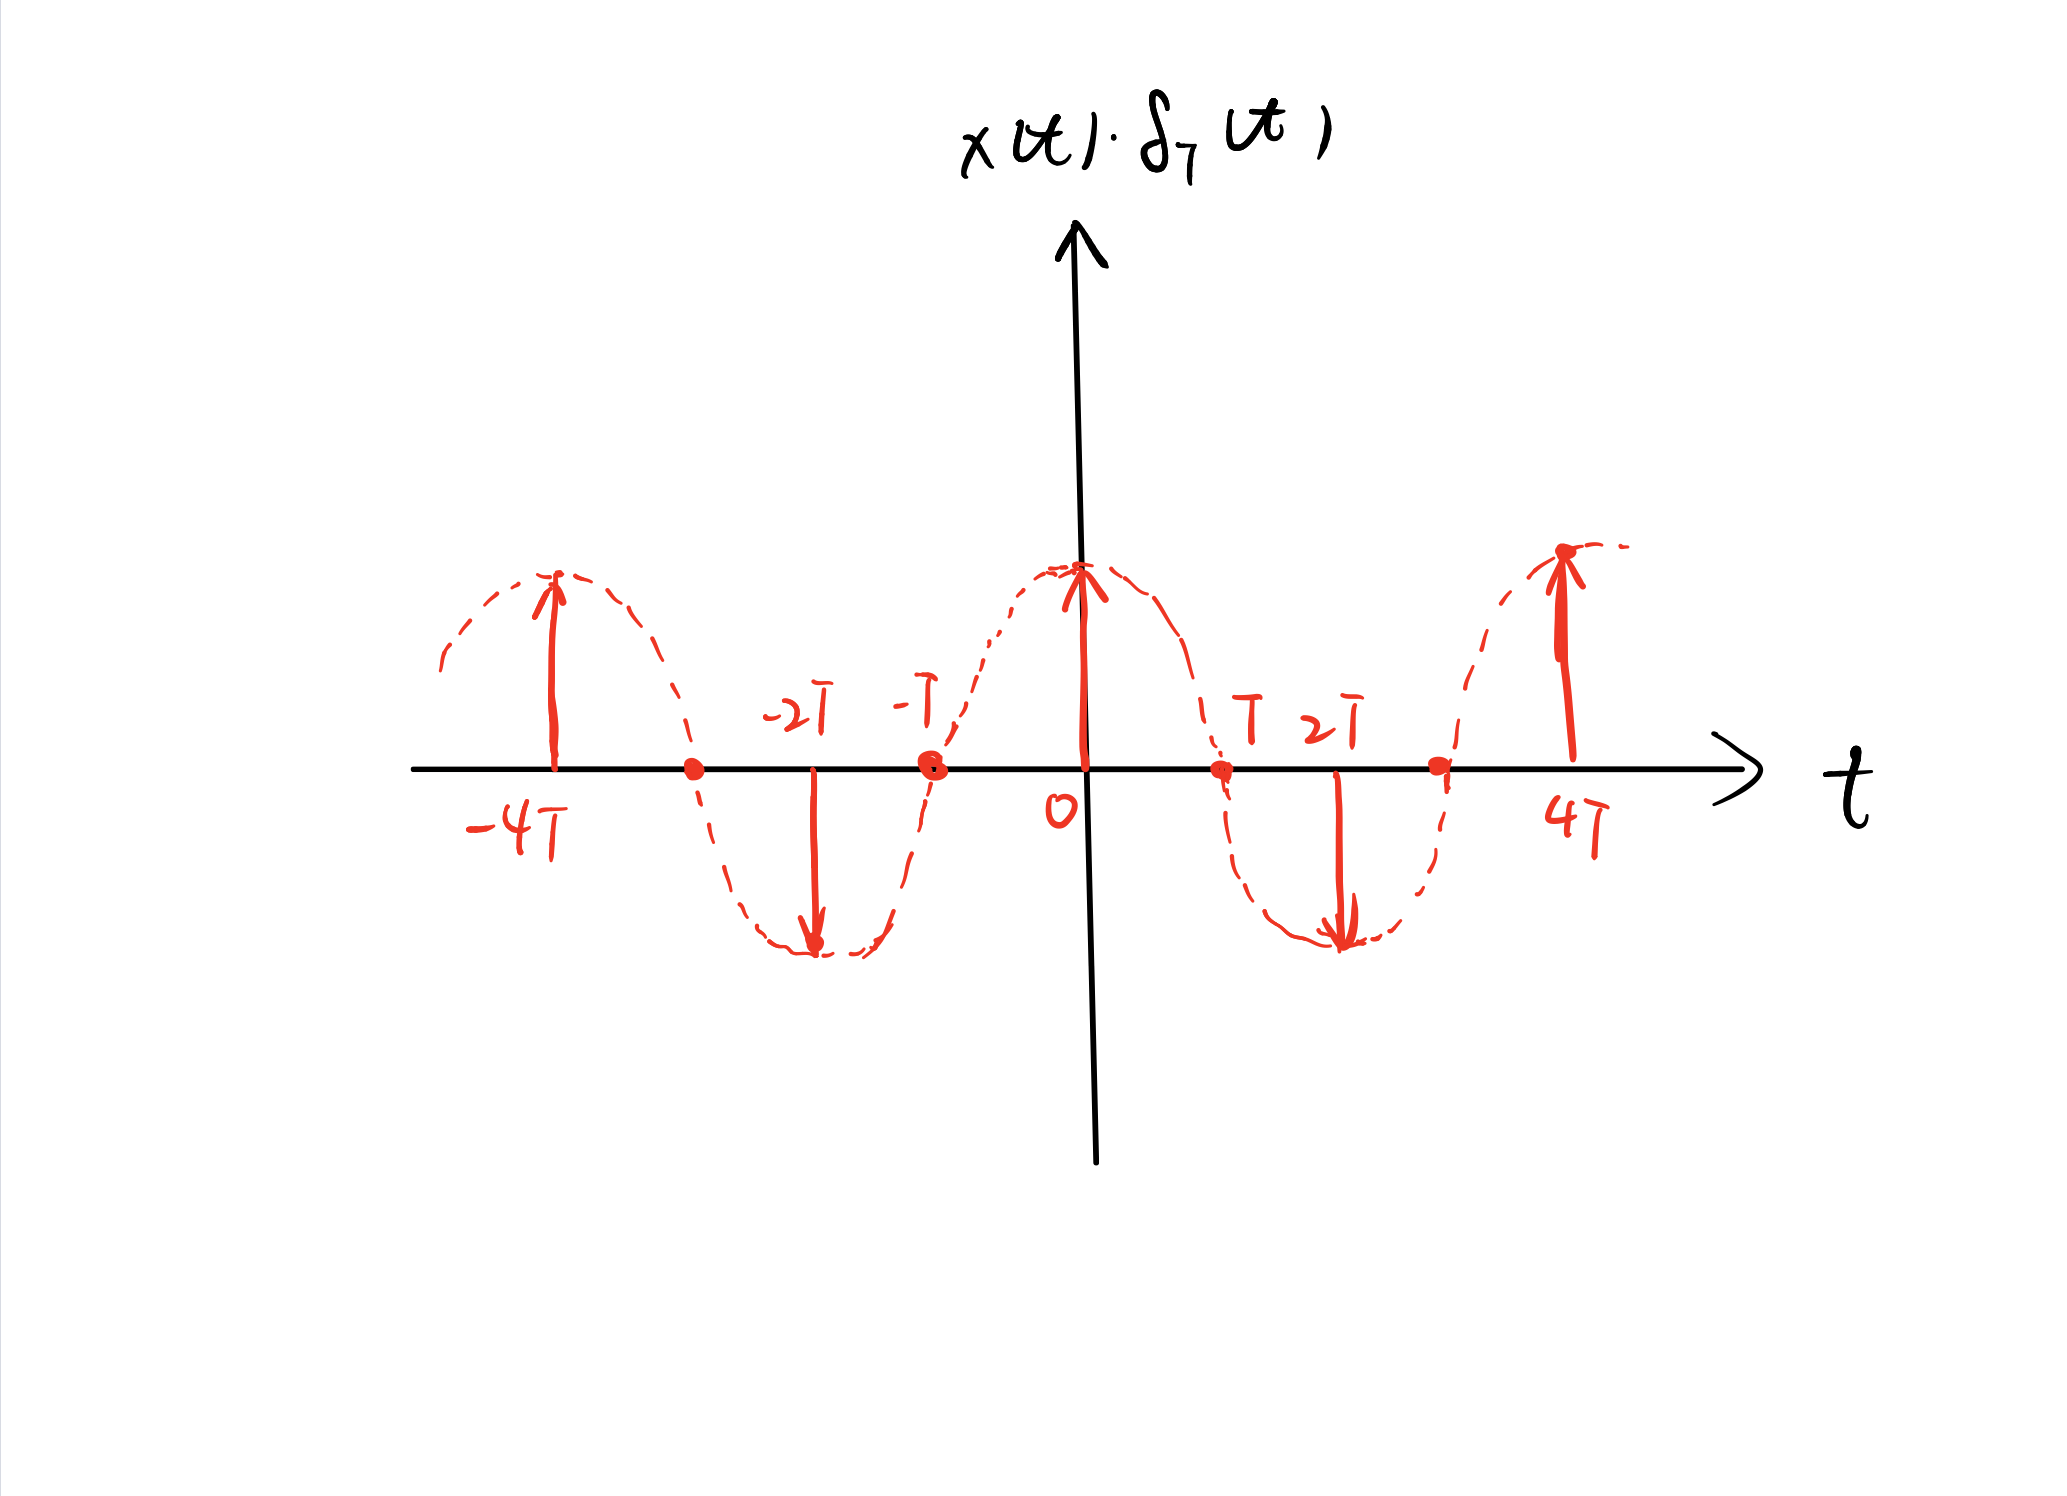
\includegraphics[width=0.8\textwidth,height=7.5cm]{pics/p2-2-1.PNG}
	\caption{(2)$x(t)\cdot\delta_T(t)$}
\end{figure}
\begin{figure}[h]
	\centering
	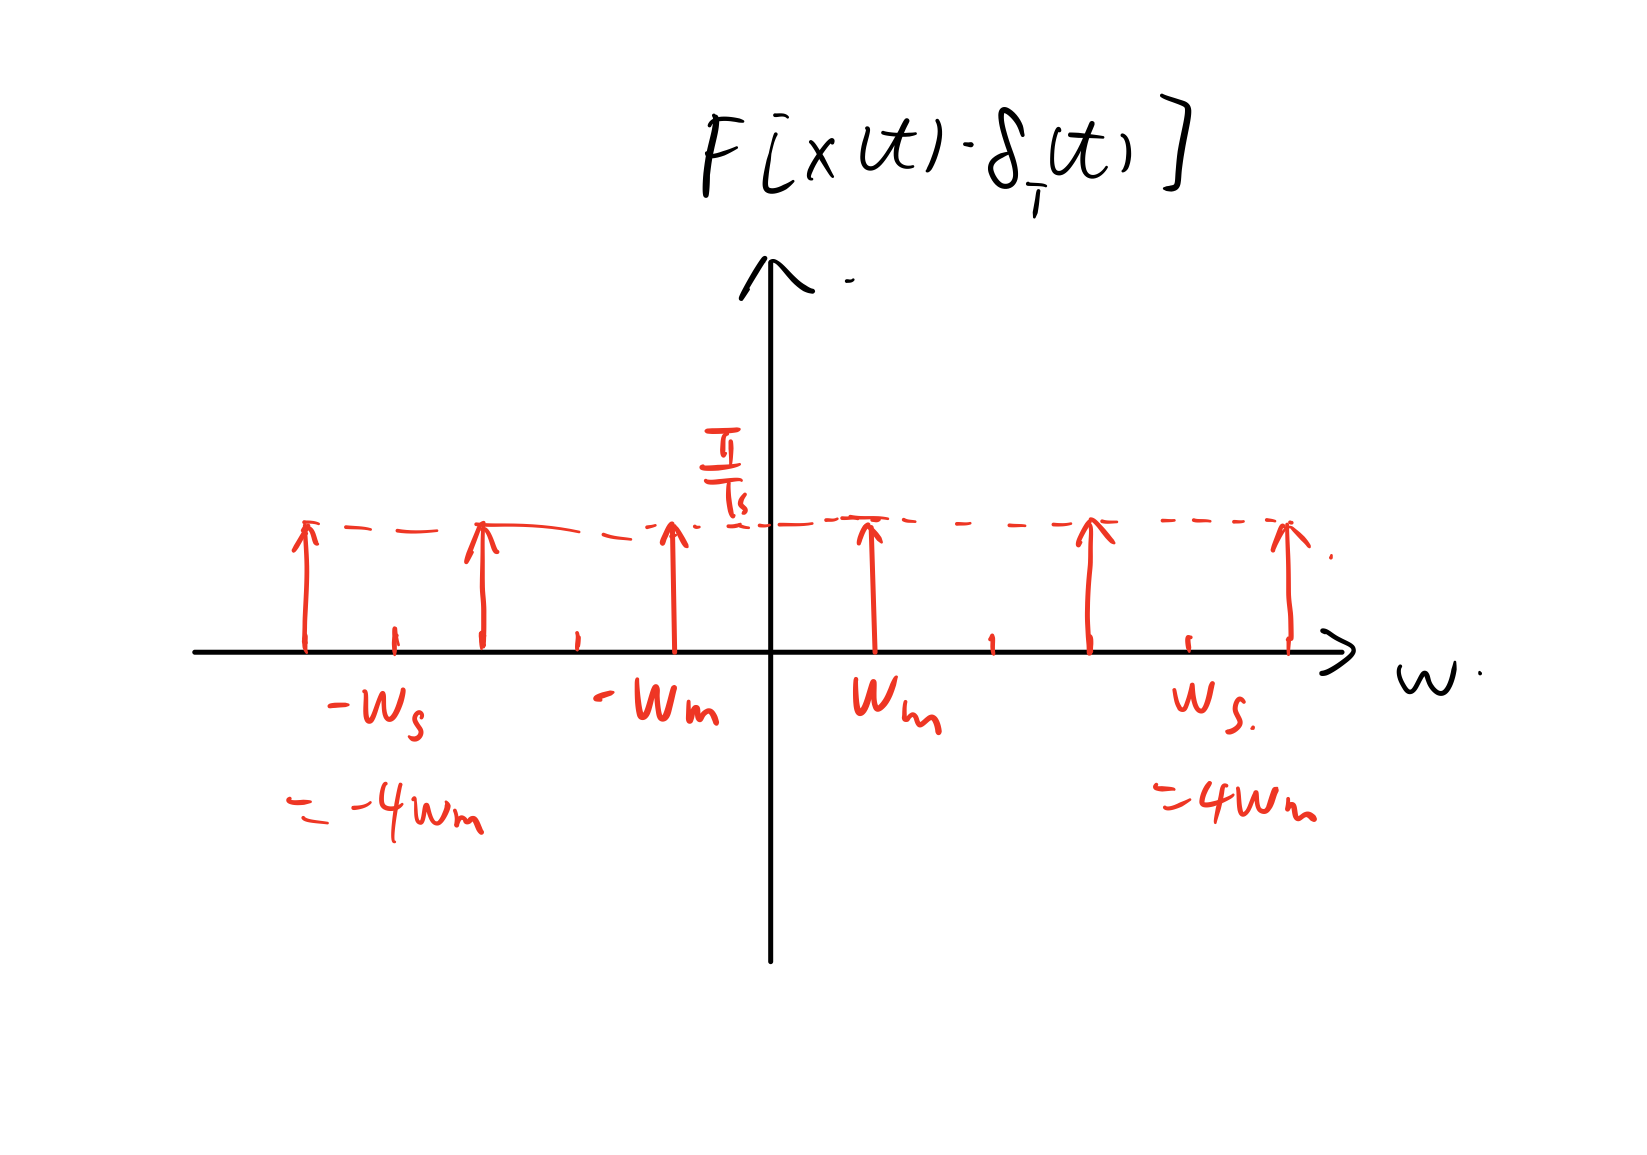
\includegraphics[width=0.8\textwidth,height=7cm]{pics/p2-2-2.PNG}
	\caption{(2)$\mathcal{F}[x(t)\delta_T(t)]$}
\end{figure}

\newpage
(3)、$x(t)$周期$T_0=\frac{2\pi}{w_m}=2T$,图片如下:\\
\begin{figure}[h]
	\centering
	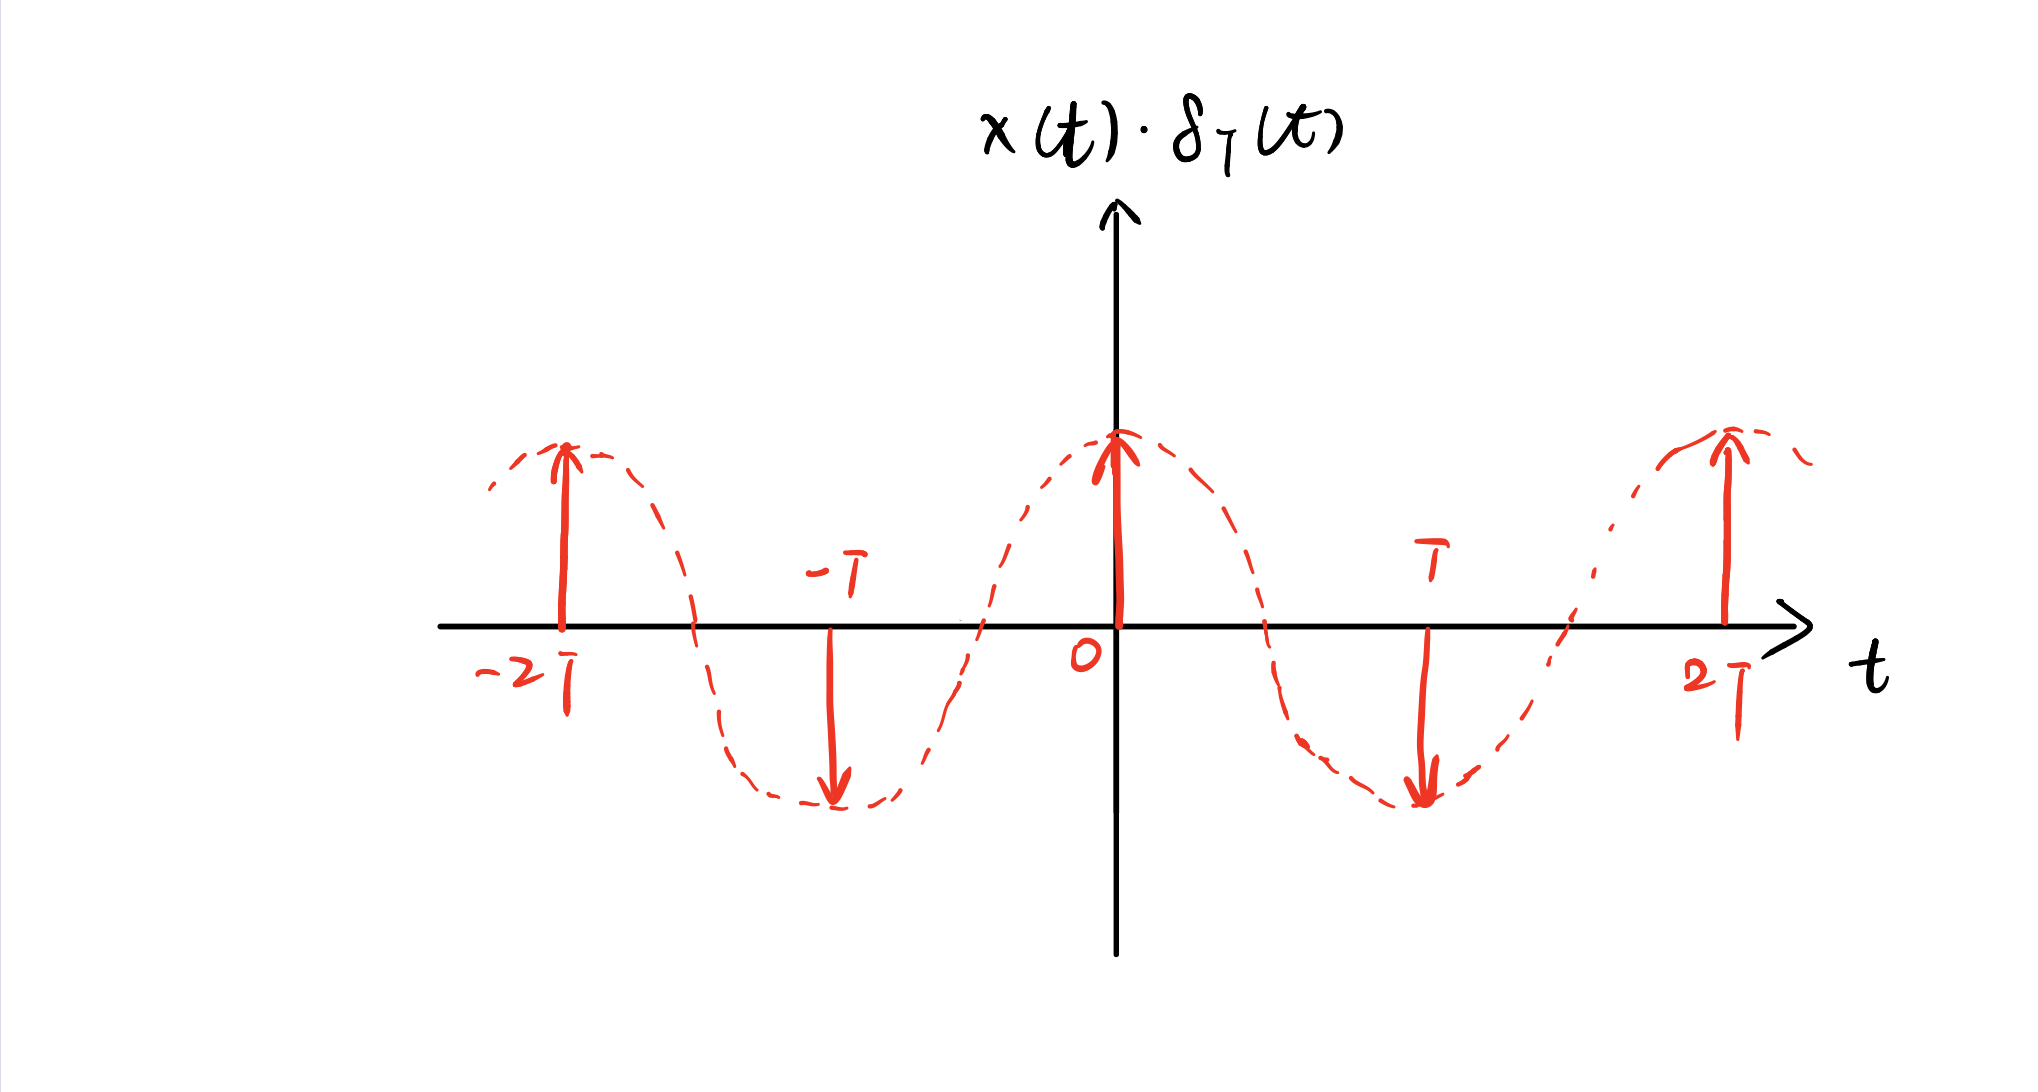
\includegraphics[width=0.8\textwidth,height=0.25\textheight]{pics/p2-3-1.PNG}
	\caption{(3)$x(t)\cdot\delta_T(t)$}
\end{figure}
\begin{figure}[h]
	\centering
	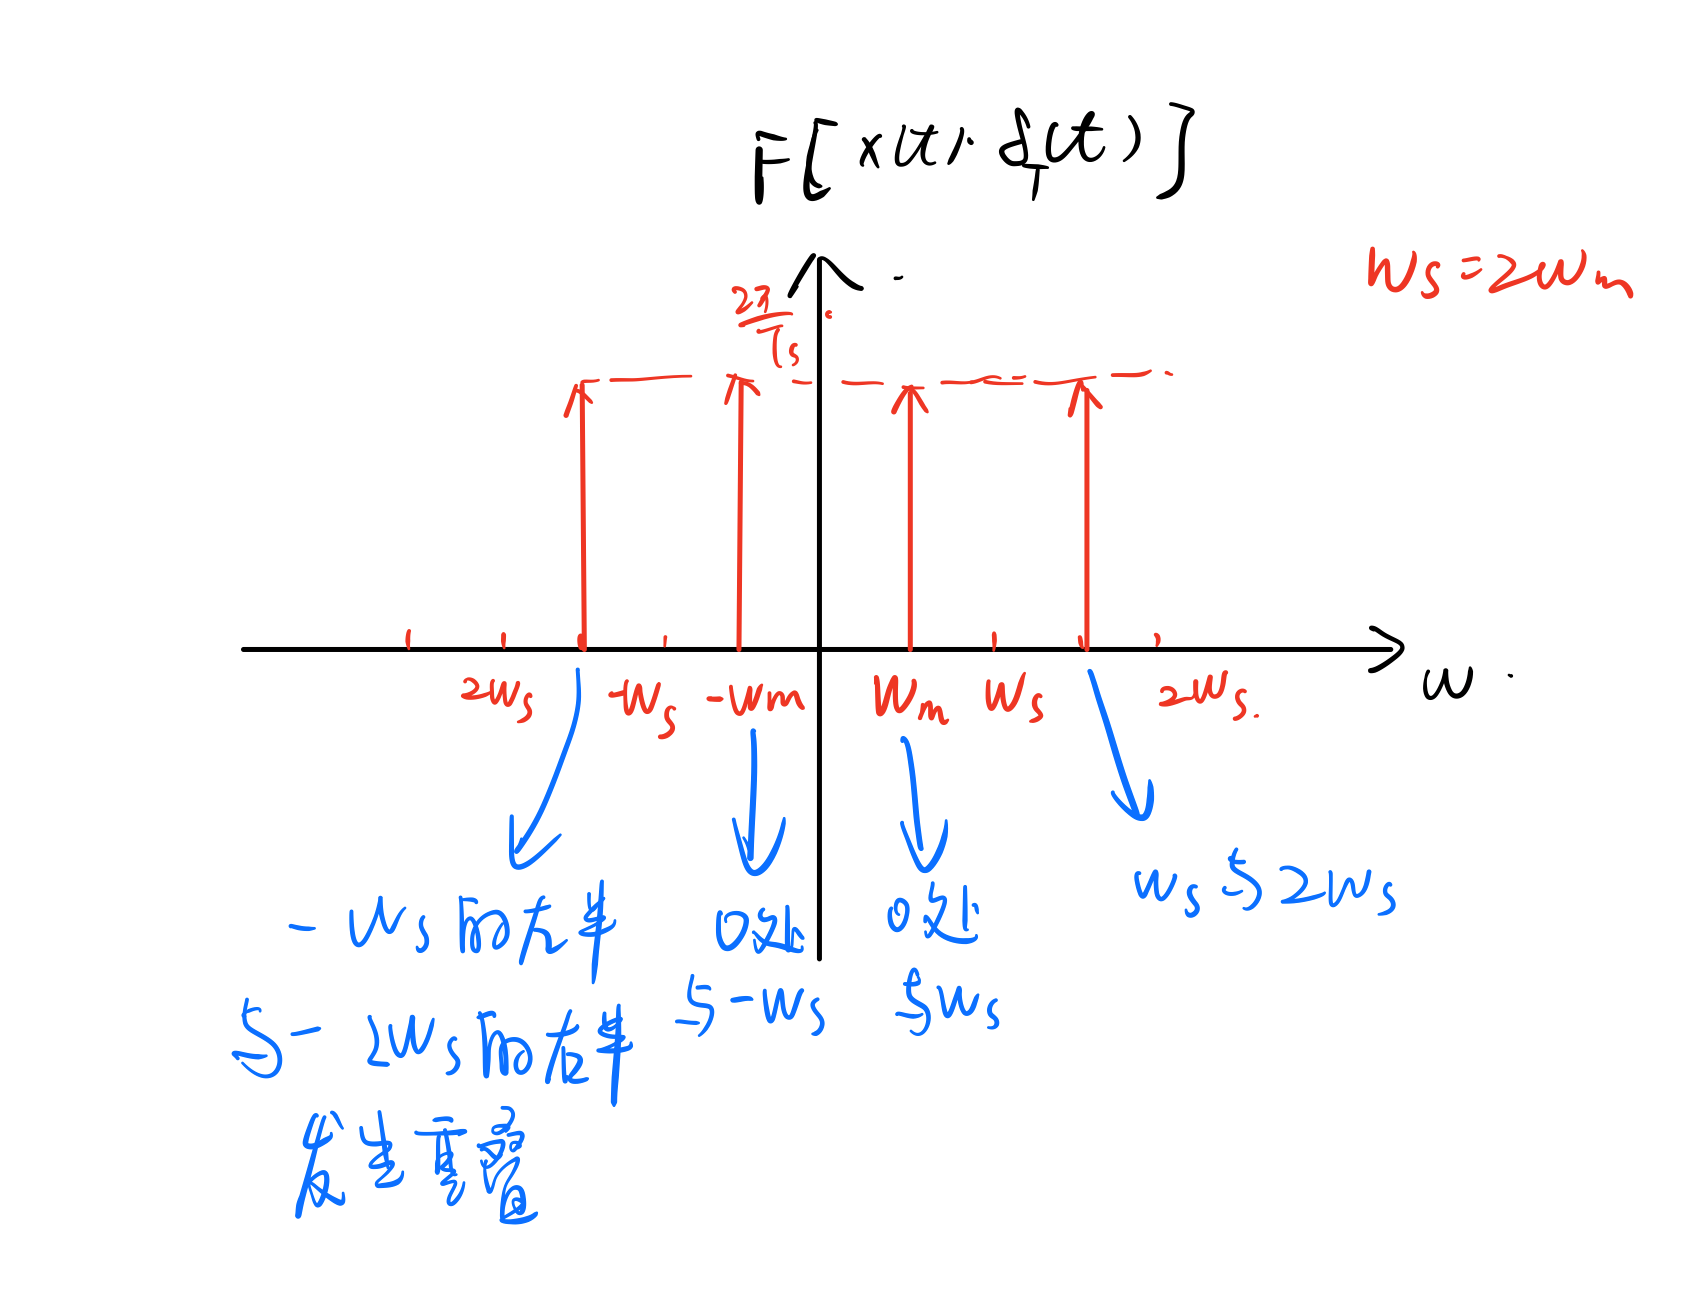
\includegraphics[width=0.8\textwidth,height=0.4\textheight]{pics/p2-3-2.PNG}
	\caption{(3)$\mathcal{F}[x(t)\cdot\delta_T(t)]$}
\end{figure}

\newpage
(4)、$x(t)$周期$T_0=\frac{2\pi}{w_m}=\frac{8}{9}T$,图片如下:\\
\begin{figure}[h]
	\centering
	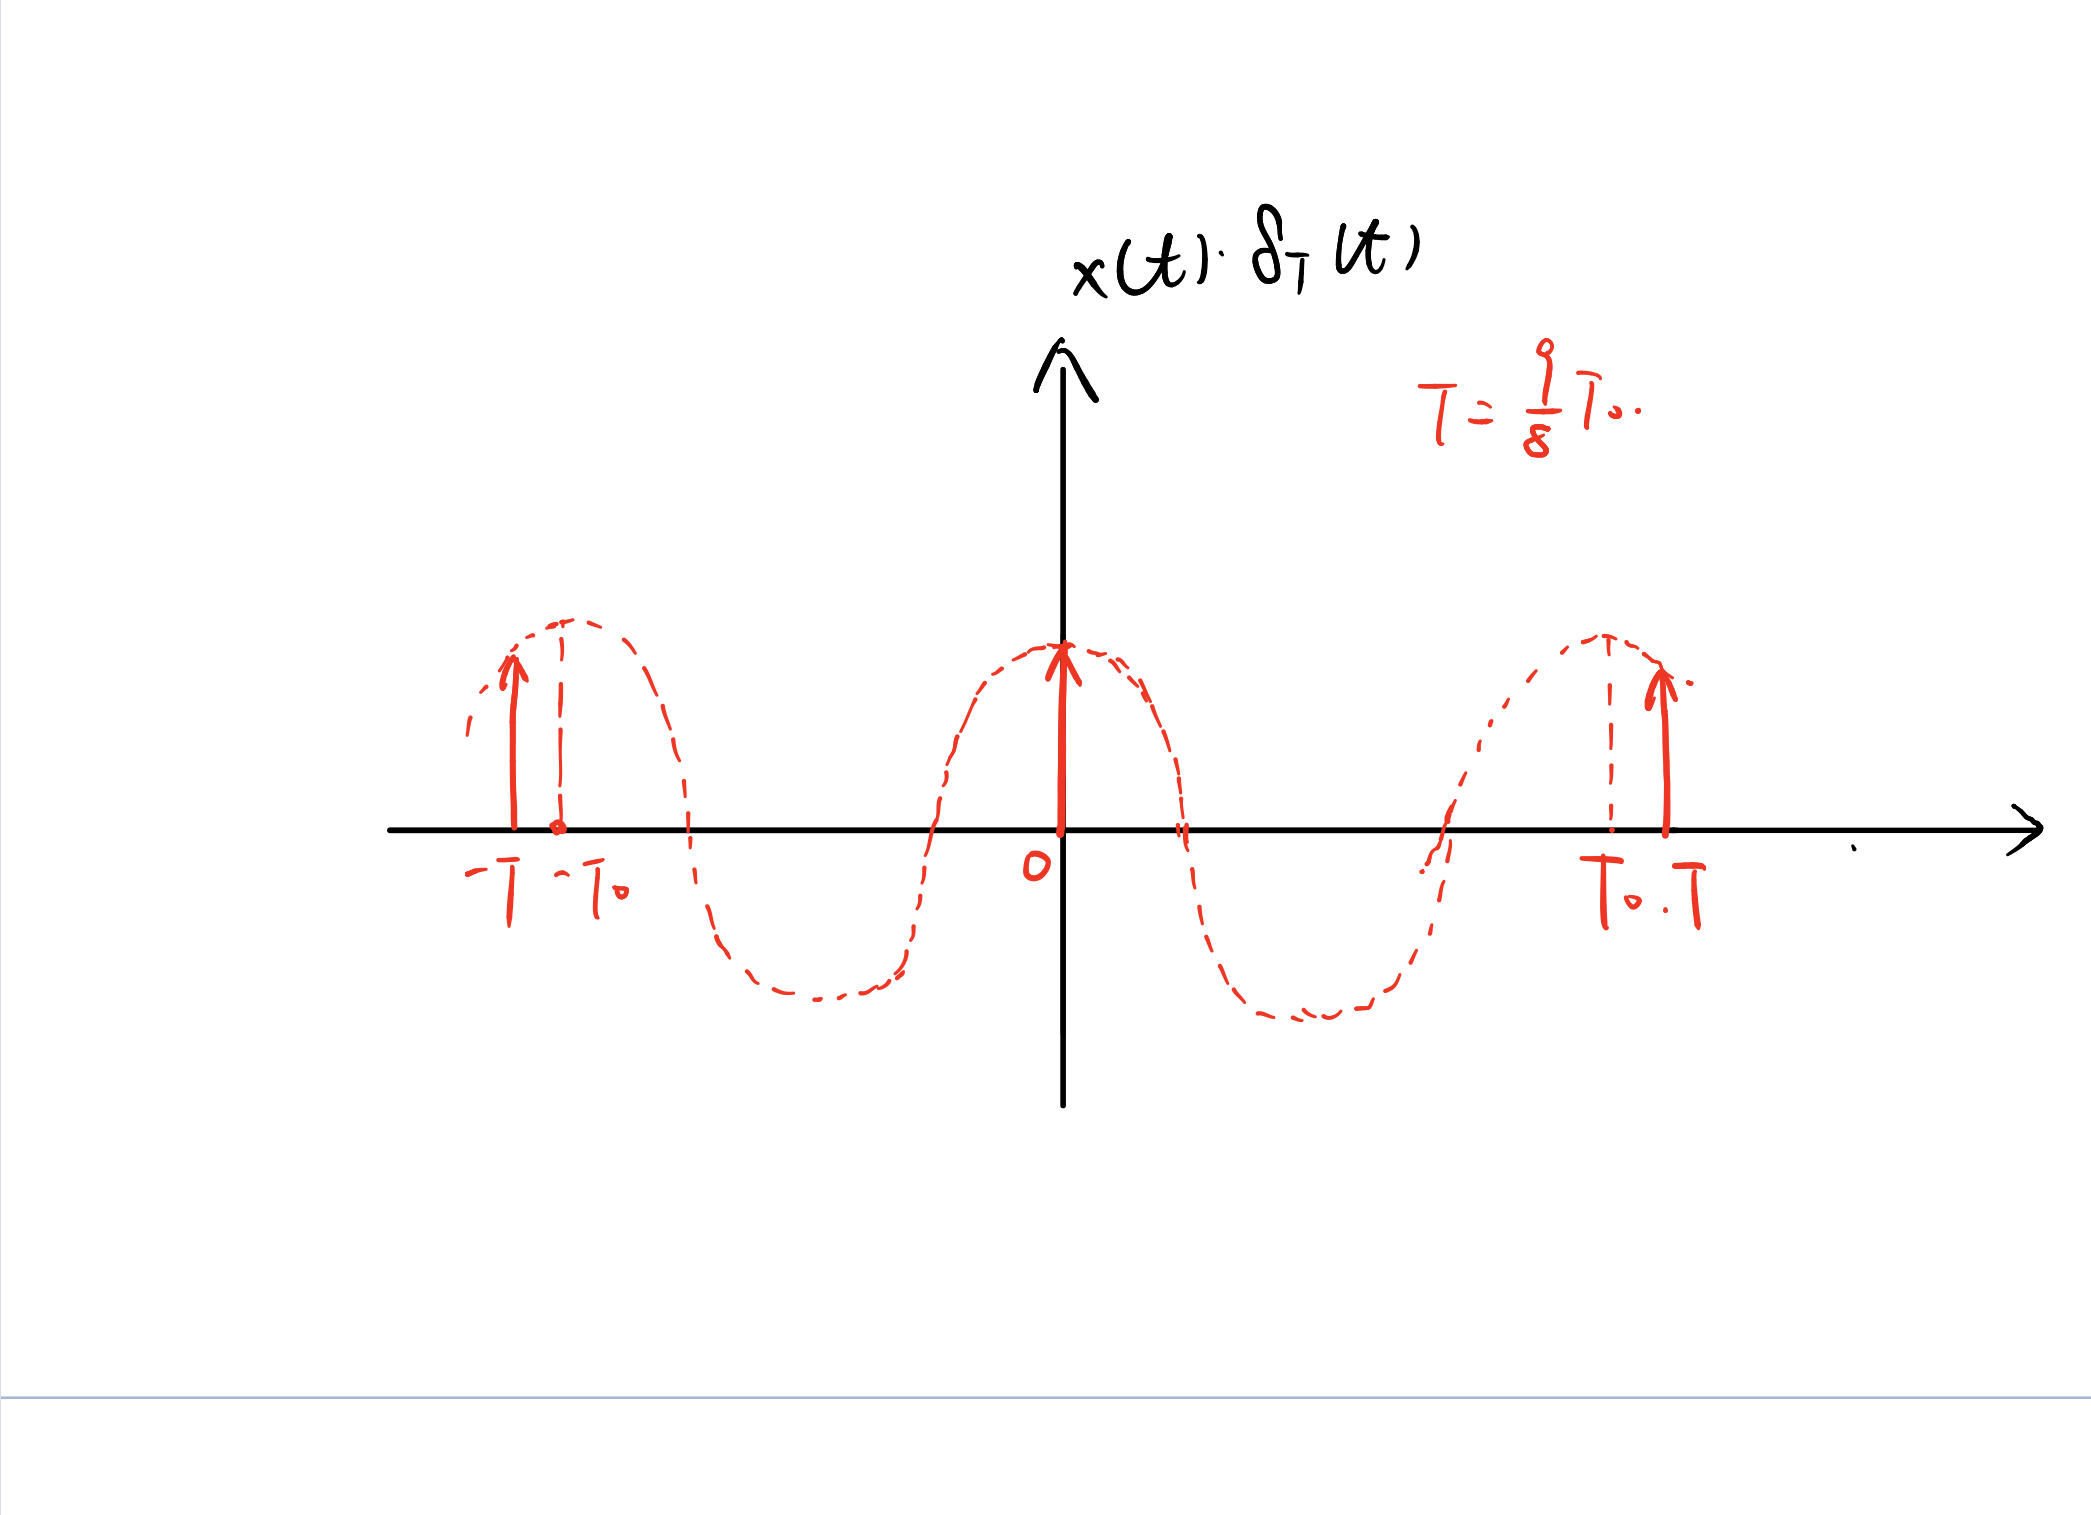
\includegraphics[width=0.8\textwidth,height=0.25\textheight]{pics/p2-4-1.PNG}
	\caption{(4)$x(t)\cdot\delta_T(t)$}
\end{figure}
\begin{figure}[h]
	\centering
	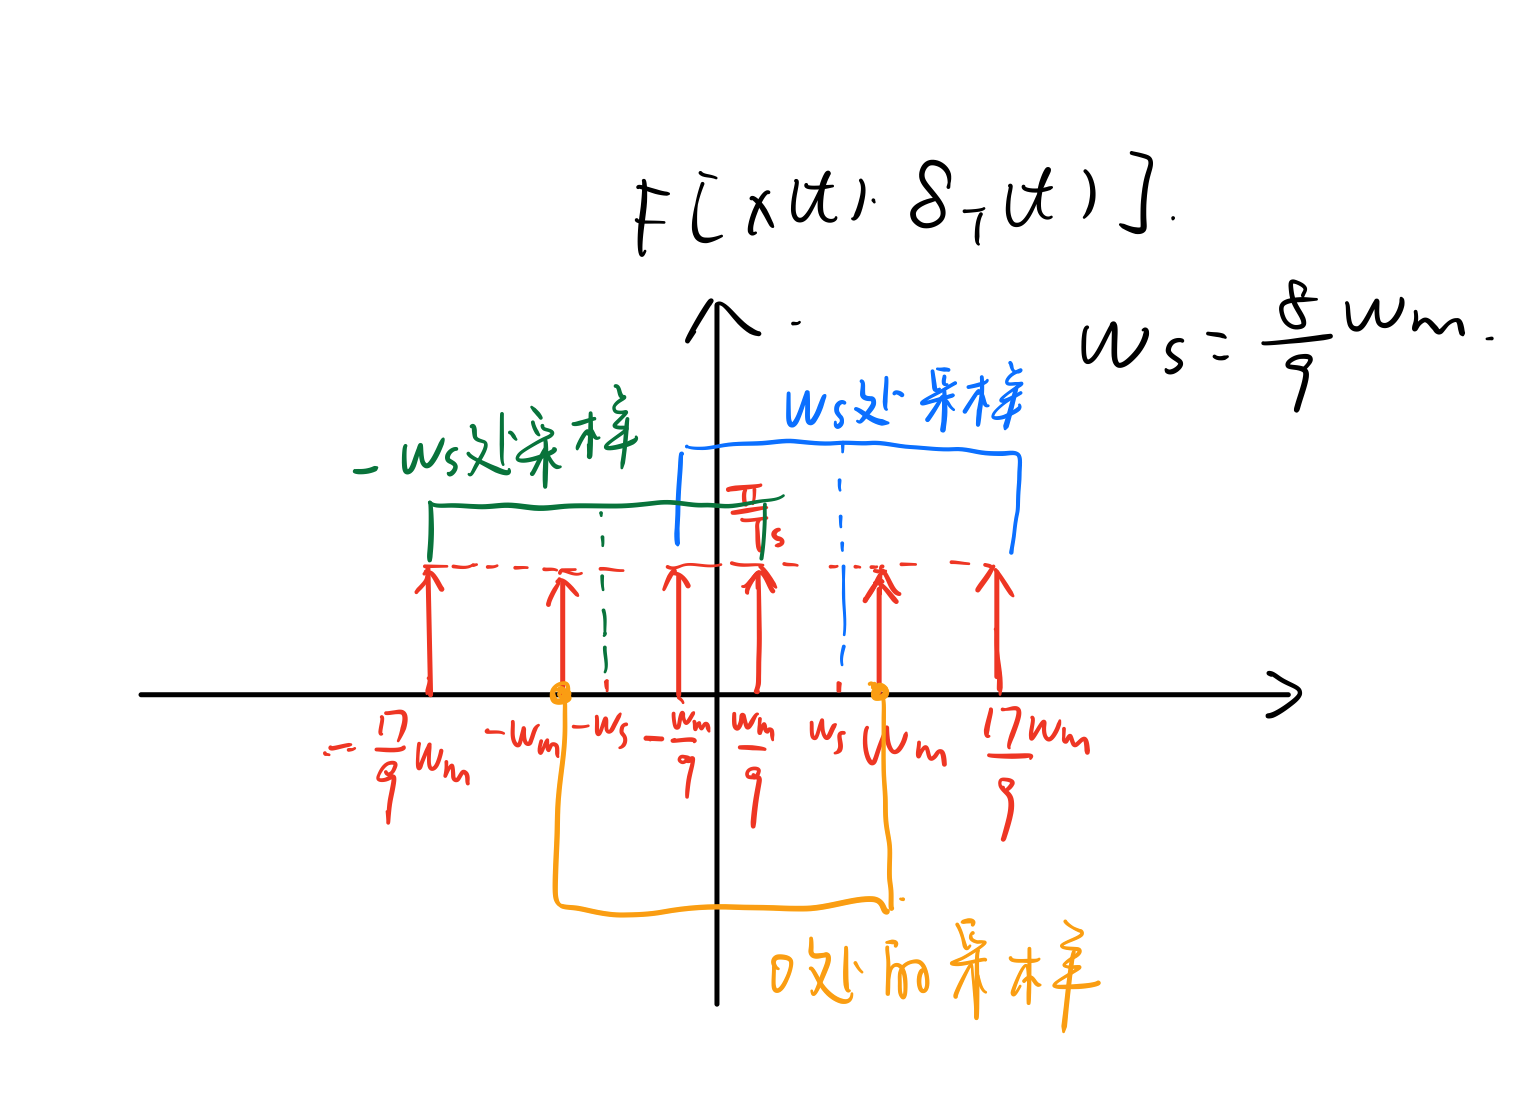
\includegraphics[width=0.8\textwidth,height=0.4\textheight]{pics/p2-4-2.PNG}
	\caption{(4)$\mathcal{F}[x(t)\delta_T(t)]$}
\end{figure}

\newpage
\question 已知信号$x(t)$的傅里叶变换为$X(\text{j}\omega)$,对$x(t)$进行冲激串采样,产生信号$x_{p}(t)=\sum_{n=-\infty}^{\infty}x(nT)\delta(t-nT)$,这里$T=10^{-4}$。对于以下所给的关于$x(t)$和(或)$X(\text{j}\omega)$的约束条件,试判断采样定理能否保证由$x_{p}(t)$恢复$x(t)$?
\begin{enumerate}[(1)]
\item 当$|\omega|>5000\pi$时,$X(\text{j}\omega)=0$
\item 当$|\omega|>15000\pi$时,$X(\text{j}\omega)=0$
\item 当$|\omega|>5000\pi$时,$\text{Re}\{X(\text{j}\omega)\}=0$
\item $x(t)$是实的,且当$\omega>5000\pi$时,$X(\text{j}\omega)=0$
\item $x(t)$是实的,且当$\omega<-15000\pi$时,$X(\text{j}\omega)=0$
\item 当$|\omega|>15000\pi$时,$X(\text{j}\omega)\ast X(\text{j}\omega)=0$
\item 当$\omega>5000\pi$时,$|X(\text{j}\omega)|=0$
\end{enumerate}

\end{questions}
\begin{solution}
	采样定理要求采样间隔$T_s<\frac{1}{2f_m}(w_s>2w_m)$,其中$2w_m$为待采样信号的频带宽度
	,由题给条件可知,采样信号的$T_s=10^{-4},w_s=20000\pi$\\
	~\\
	(1)能\\
	因为条件意味着$w_m=5000\pi$,而$w_s=20000\pi>2w_m$\\
	~\\
	(2)不能\\
	条件意味着$w_m=15000\pi$,而$w_s=20000\pi<2w_m$,\\无法保证$(10000\pi,15000\pi),(-10000\pi,-15000\pi)$上$X(jw)=0$\\
	~\\
	(3)能\\
	时域信号的实部对应频域中的偶对称实部和奇对称虚部\\
	时域信号的虚部对应频域中的奇对称实部和偶对称虚部\\
	故通过条件可知$w_m=5000\pi$,后续同(1)\\
	~\\
	(4)能\\
	因为实信号的频谱是对称的,所以条件意味着$w_m=5000\pi$,后续同(1)\\
	~\\
	(5)不能\\
	无法保证$(-10000\pi,-15000\pi)$上$X(jw)=0$\\
	~\\
	(6)能\\
	$\mathcal{F}[x(t)\cdot x(t)]=\frac{1}{2\pi}[X(jw)*X(jw)]$\\
	设频带宽度为$2w_m$,则$X(jw)*X(jw)$的频带宽度为$4w_m$,\\
	由题给条件可知$30000\pi=4w_m\rightarrow w_m=7500\pi$,故$w_s>2w_m$\\
	~\\
	(7)不能\\
	由题目条件知,$w>5000\pi$时,频谱的实部和虚部均为0,\\
	对于实信号,显然有$w_m=5000\pi$\\
	对于复信号,其频谱实部由一个偶对称部分和一个奇对称部分组成,\\
	在$w>5000\pi$的时候有$X_{\mbox{偶对称}}(jw)+X_{\mbox{奇对称}}(jw)=0$,\\
	但是到了$w<-5000\pi$的时候,由于偶对称和奇对称的特性,二者叠加不再为0,
	这也就意味着无法得到确切的$w_m$,故无法保证满足采样定理
\end{solution}
\end{document}